\begin{center}
	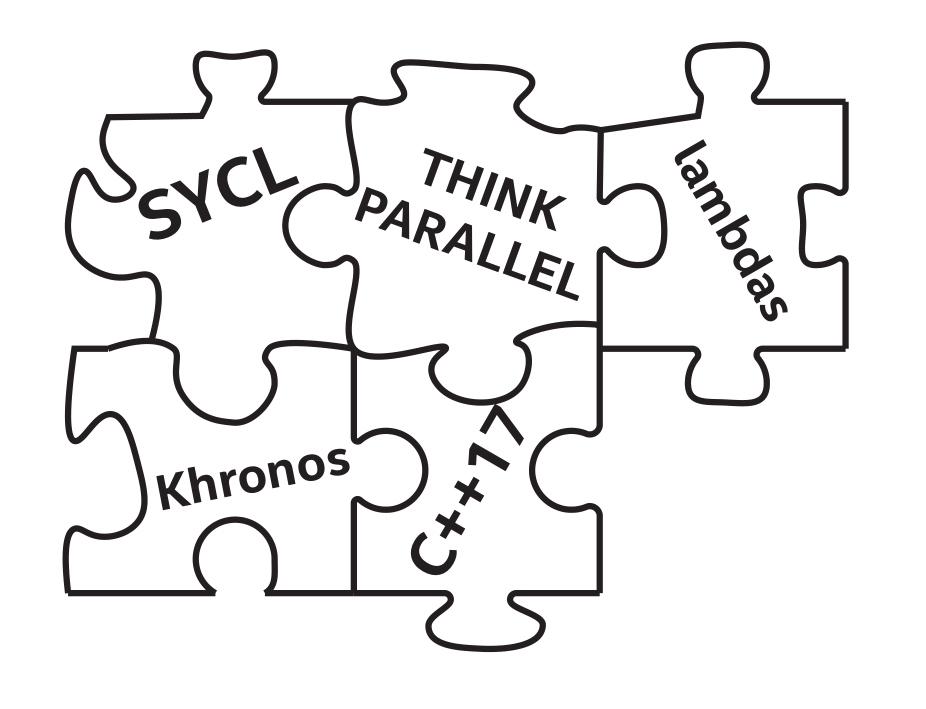
\includegraphics[width=0.5\textwidth]{content/chapter-1/images/1}
\end{center}

本章通过介绍核心概念(包括术语)来奠定基础,这些概念在学习C++数据并行加速时非常重要。\par

C++中的数据并行性,允许现代异构系统并行访问资源。C++应用程序可以使用任何设备的组合——包括GPU、CPU、FPGA和AI专用硬件(ASIC)——以便解决当前的问题。\par

在这本书中会学到如何使用C++和SYCL进行数据并行编程。\par

SYCL(发音为sickle)是一个行业驱动的Khronos标准,它为异构系统在C++中增加了数据并行性。SYCL程序与支持SYCL的C++编译器(如本书中使用的开源数据并行C++(DPC++)编译器)一起使用时,性能最好。SYCL不是首字母缩写,SYCL只是一个名字。\par

DPC++是一个开源编译器项目,最初由Intel创建,致力于支持C++中的数据并行。DPC++编译器基于SYCL、一些扩展和异构支持,包括GPU、CPU和FPGA设备。除了DPC++的开源版本,还有Intel oneAPI工具包中的商业版本。\par

DPC++编译器的开源版本和商业版本都支持基于SYCL的实现特性。本书中的所有例子都可以使用DPC++编译器的任何一个版本进行编译,而且所有的例子都可以使用最新的SYCL编译器进行编译。发布时,我们会特别注意使用DPC++扩展的地方。\par

